\documentclass[12pt,a4paper]{article}

\setlength{\textwidth}{165mm}
\setlength{\textheight}{240mm}
\setlength{\parindent}{0mm} % S{\aa} meget rykkes ind efter afsnit
\setlength{\parskip}{\parsep}
\setlength{\headheight}{0mm}
\setlength{\headsep}{0mm}
\setlength{\hoffset}{-2.5mm}
\setlength{\voffset}{0mm}
\setlength{\footskip}{15mm}
\setlength{\oddsidemargin}{0mm}
\setlength{\topmargin}{0mm}
\setlength{\evensidemargin}{0mm}
\usepackage{multicol}
\usepackage{blindtext}
\usepackage[all]{xy}
\usepackage{graphicx}    % For grafik (billederfiler)
\usepackage[T1]{fontenc} % For at blande \textsc{} med \textbf{}
\usepackage[utf8]{inputenc}
\usepackage{amsfonts,amsmath,amssymb}
\usepackage{eucal}
\usepackage{enumerate}  
\usepackage{hyperref}
\usepackage{url}
\usepackage{mathptmx}
\usepackage{multirow}
\usepackage[dvipsnames,usenames]{color}
\usepackage{tabularx,colortbl,xcolor}
\usepackage{listings}
\usepackage{color}
\usepackage{amsmath}
\usepackage{xcolor}

\definecolor{KU-red}{RGB}{144,26,30} 
\definecolor{dkgreen}{rgb}{0,0.6,0}
\definecolor{gray}{rgb}{0.5,0.5,0.5}
\definecolor{mauve}{rgb}{0.58,0,0.82}

\lstset{frame=tb,
  language=Java,
  aboveskip=3mm,
  belowskip=3mm,
  showstringspaces=false,
  columns=flexible,
  basicstyle={\small\ttfamily},
  numbers=none,
  numberstyle=\tiny\color{gray},
  keywordstyle=\color{blue},
  commentstyle=\color{dkgreen},
  stringstyle=\color{mauve},
  breaklines=true,
  breakatwhitespace=true,
  tabsize=3}

\DeclareSymbolFont{usualmathcal}{OMS}{cmsy}{m}{n}
\DeclareSymbolFontAlphabet{\mathcal}{usualmathcal}
\DeclareSymbolFont{letters}{OML}{txmi}{m}{it}

\DeclareMathSymbol{\alpha}{\mathord}{letters}{"0B}
\DeclareMathSymbol{\beta}{\mathord}{letters}{"0C}
\DeclareMathSymbol{\gamma}{\mathord}{letters}{"0D}
\DeclareMathSymbol{\delta}{\mathord}{letters}{"0E}
\DeclareMathSymbol{\epsilon}{\mathord}{letters}{"0F}
\DeclareMathSymbol{\zeta}{\mathord}{letters}{"10}
\DeclareMathSymbol{\eta}{\mathord}{letters}{"11}
\DeclareMathSymbol{\theta}{\mathord}{letters}{"12}
\DeclareMathSymbol{\iota}{\mathord}{letters}{"13}
\DeclareMathSymbol{\kappa}{\mathord}{letters}{"14}
\DeclareMathSymbol{\lambda}{\mathord}{letters}{"15}
\DeclareMathSymbol{\mu}{\mathord}{letters}{"16}
\DeclareMathSymbol{\nu}{\mathord}{letters}{"17}
\DeclareMathSymbol{\xi}{\mathord}{letters}{"18}
\DeclareMathSymbol{\pi}{\mathord}{letters}{"19}
\DeclareMathSymbol{\rho}{\mathord}{letters}{"1A}
\DeclareMathSymbol{\sigma}{\mathord}{letters}{"1B}
\DeclareMathSymbol{\tau}{\mathord}{letters}{"1C}
\DeclareMathSymbol{\upsilon}{\mathord}{letters}{"1D}
\DeclareMathSymbol{\phi}{\mathord}{letters}{"1E}
\DeclareMathSymbol{\chi}{\mathord}{letters}{"1F}
\DeclareMathSymbol{\psi}{\mathord}{letters}{"20}
\DeclareMathSymbol{\omega}{\mathord}{letters}{"21}
\DeclareMathSymbol{\varepsilon}{\mathord}{letters}{"22}
\DeclareMathSymbol{\vartheta}{\mathord}{letters}{"23}
\DeclareMathSymbol{\varpi}{\mathord}{letters}{"24}
\DeclareMathSymbol{\varrho}{\mathord}{letters}{"25}
\DeclareMathSymbol{\varsigma}{\mathord}{letters}{"26}
\DeclareMathSymbol{\varphi}{\mathord}{letters}{"27}
\DeclareMathSymbol{\Gamma}{\mathord}{letters}{"00}
\DeclareMathSymbol{\Delta}{\mathord}{letters}{"01}
\DeclareMathSymbol{\Theta}{\mathord}{letters}{"02}
\DeclareMathSymbol{\Lambda}{\mathord}{letters}{"03}
\DeclareMathSymbol{\Xi}{\mathord}{letters}{"04}
\DeclareMathSymbol{\Pi}{\mathord}{letters}{"05}
\DeclareMathSymbol{\Sigma}{\mathord}{letters}{"06}
\DeclareMathSymbol{\Upsilon}{\mathord}{letters}{"07}
\DeclareMathSymbol{\Phi}{\mathord}{letters}{"08}
\DeclareMathSymbol{\Psi}{\mathord}{letters}{"09}
\DeclareMathSymbol{\Omega}{\mathord}{letters}{"0A}
\DeclareMathSymbol{\upGamma}{\mathalpha}{operators}{"00}
\DeclareMathSymbol{\upDelta}{\mathalpha}{operators}{"01}
\DeclareMathSymbol{\upTheta}{\mathalpha}{operators}{"02}
\DeclareMathSymbol{\upLambda}{\mathalpha}{operators}{"03}
\DeclareMathSymbol{\upXi}{\mathalpha}{operators}{"04}
\DeclareMathSymbol{\upPi}{\mathalpha}{operators}{"05}
\DeclareMathSymbol{\upSigma}{\mathalpha}{operators}{"06}
\DeclareMathSymbol{\upUpsilon}{\mathalpha}{operators}{"07}
\DeclareMathSymbol{\upPhi}{\mathalpha}{operators}{"08}
\DeclareMathSymbol{\upPsi}{\mathalpha}{operators}{"09}
\DeclareMathSymbol{\upOmega}{\mathalpha}{operators}{"0A}

\newcommand{\hhemail}[1]{\textsf{#1}}
\newcommand{\hhurl}[1]{{\color{blue}\url{#1}}}

\begin{document}
	
	\begin{minipage}[b]{1.0\linewidth} 
				
\includegraphics[height=50mm]{KULogo.pdf}
		
		\vspace*{-16ex}
		\vspace {35ex}
		\begin{center}
			{\huge \bf Project: Beetle} \vspace*{4ex} \\
			{\large 22. april 2015}\\
			\vspace*{2ex}
			qzj710 - 121095 - Enes Golic \\
			rpc308 - 070493 - Yunus Emre Okutan \\
			cbh239 - 250594 - Casper Lützhøft Christensen \\
			mhb558 - 250795 - Tor-Salve Dalsgaard\\
			\vspace*{1ex}
			Instructor - Kasper Passov
			
		\end{center}
	\end{minipage}
	
\newpage
\tableofcontents

\newpage
\section{Introduction}
\subsection{Abstract}
Our project is, in broad terms, a search-engine for insects, which is to be provided to our client, the University of Hamburg.\\
Through German law and regulation, it is specified that in order for a university to receive governmental funding, it must allow public access to the research done by the specific university, and it is this context our project is necessary.\\
The entomology department of the University of Hamburg has a catalogue of information on different insects, their names, species, genus and a picture of the insect’s anatomy.\\
This information needs to be available to the public, and the University of Hamburg wishes this done through the usage of a search-engine connected to a database.\\
The database must contain the insects as entries, with their names, species, genus and anatomy-pictures as attributes. The search-engine must then allow a visitor to input a search-term, which will be tried against any of the database’s attributes, and return any entry that matches the search-term.
It must also contain an advanced search-function that allows you to match a specific term to a specific attribute.\\
Furthermore, the University of Hamburg requires a method through which they can update the database themselves. Both to allow them to edit entries that may contain errors and to add/remove entries to/from the database. This method must only be available to authorised employees and not at all available to visitors on the website. \\
We are creating the search-engine in PHP, and it is to be implemented onto their website. The database is being created in MySQL and it will be editable through a method created either in PHP and implemented onto the website itself, or a stand-alone program, created in Java, given to the authorised people.\\

\newpage

\section{FACTOR}
\subsection{Functionality}
Allow visitors to use the 2 search-functions, basic and advanced, to search through a database of insect-entries with data collected by the University of Hamburg.
Allow employees with the necessary login credentials to edit the database to either remove entries, change existing entries or add new entries.
\subsection{Application-domain}
Allow free, public access of data collected through research done by the University of Hamburg, so that everyone may learn from the conducted research.
\subsection{Conditions}
The product is being developed as part of the course PKSU at the University of Copenhagen. It is done entirely voluntarily and is non-profit. The client's wishes to the product are all taken into account and will be attempted fulfilled, although no complete product can be expected.
\subsection{Technology}
The product is developed on completely normal personal computers - no special tools are necessary in development apart from a PC.
The product is designed to run in any browser without any necessary plugins, meaning that nothing but a PC and a working internet connection is required to use the product.
\subsection{Objects}
Anonymous visitors and employees can respectively view and edit the database entries.
\subsection{Responsibility}
The responsibility of the product is, through a search-engine, to ensure free and public access to research conducted by the University of Hamburg. 
\newpage
\section{Program Specifications}
\subsection{Functional and Non-Functional Requirements}

If we refer to the abstract outlining the program's specifications, we get a general feel of the architecture of the software and how it is going to work. Drawing on those points we can, for the sake of overview, specify functional and non-functional requirements for the program.\\

{\bf Functional Requirements}
\begin{itemize}
	\item The product must offer a search-option that returns any and every entry that contains an attribute that matches the search input.
	\item The product must offer a search-option that allows matching of specific search-inputs to specific attributes and return any and every entry that matches the terms in their specific attributes.
	\item The database must allow the creation of new entries, editing of existing entries and deletion of existing entries.
	\item The database must be unable to be edited by anyone save the authorised employees.
	\item A fitting message must be displayed if no matching entries are found.\\
\end{itemize}
{\bf Non-Functional Requirements}
\begin{itemize}
	\item The search-engine must be developed in PHP so it can run on their website in any browser with no additional requirements.
	\item The method of editing the database must be simple enough for people without pre-existing IT skills to use it.
	\item The product in its finished state must look nice and fit with the colour-scheme already present on the University of Hamburg's website.
\end{itemize}
\newpage
\subsection{Use Case Model}
\vskip\medskipamount % or other desired dimension
\leaders\vrule width \textwidth\vskip0.4pt % or other desired thickness
\vskip\medskipamount % ditto
\nointerlineskip
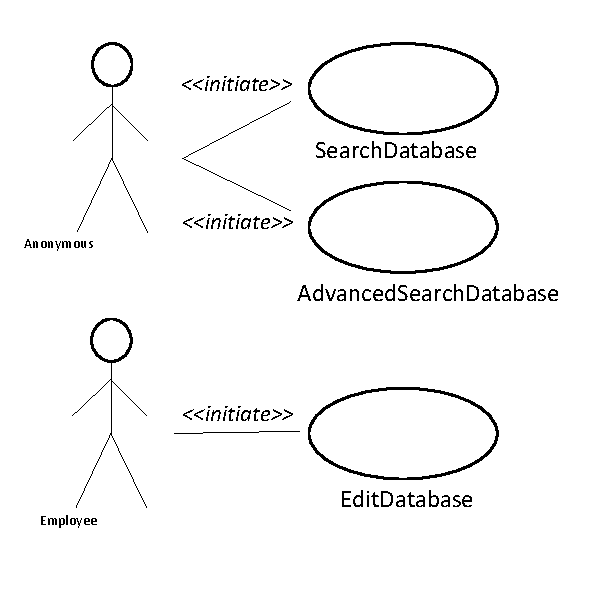
\includegraphics[height=120mm]{UseCaseModel.pdf}

{\bf SearchDatabase}\\ 
Anonymous users use the search-engine and input a term in other to search the database and have the results they require displayed.
Searching the database does not require any special permissions.

{\bf AdvancedSearchDatabase}\\
Anonymous users use the advanced search-engine and input their search-terms into the fields representing the attributes they wish to match them against, in order to have the results they require displayed.
Searching the database does not require any special permissions.

{\bf EditDatabase}\\
An employee edits the database by accessing the edit-page through entering the necessary login credentials, modifies the database in which way desired and updates the database.
EditDatabase cannot be used without valid login credentials.\\
\vskip\medskipamount % or other desired dimension
\leaders\vrule width \textwidth\vskip0.4pt % or other desired thickness
\vskip\medskipamount % ditto
\nointerlineskip
The figure above is a use case model, which showcases the different possibilties of the product and to which kind of users they are available.

It is for instance evident through the model and the description of the functions, that any user will be able to search the database both in a basic and advanced way, where as only an employee with the necessary login credentials will be able to edit the entries in the database.
\newpage

\subsection{Specific Use Cases}

With the use case model created, we have an overview of the functional architecture of the website. With that in mind, we can explore some of the specific cases a bit further:\\

$\begin{array}{ll}
\hline
\text{Use Case Name}	& \text{SearchDatabase}\\
\hline
\text{Participating
	actors}	& \text{Initiated by Anonymous}\\
\hline
\text{Flow of events}	& \text{1. An anonymous user enters the website.}\\
& \text{2. The anonymous user enters the search-term into the search-field and presses send.} \\
& \text{3. The matching results are displayed.}\\
\hline
\text{Entry condition}	& \text{None}\\
\hline
\text{Exit conditions}	& \bullet \text{Anonymous exits the site.}\\
& \bullet \text{Anonymous submits a new search term.}\\
\hline
\end{array}$
\\

The above use case is the ordinary search of the database. It showcases in detail the specifics of the use case by displaying who initiates it, who, if any, it communicates with, the flow of the case itself as well as any conditions necessary.
We will now also inspect the remaining 2 use cases:\\

$\begin{array}{ll}
\hline
\text{Use Case Name}	& \text{AdvancedSearchDatabase}\\
\hline
\text{Participating
	actors}	& \text{Initiated by Anonymous}\\
\hline
\text{Flow of events}	& \text{1. An anonymous user enters the website.}\\
& \text{2. The anonymous user enters the search-terms into the fields of the matching attributes} \\
& \text{and presses send.}\\
& \text{3. The matching results are displayed.}\\
\hline
\text{Entry condition}	& \text{None}\\
\hline
\text{Exit conditions}	& \bullet \text{Anonymous exits the site.}\\
& \bullet \text{Anonymous submits a new search term.}\\
\hline
\end{array}$\\
\\
As we can see in the above case, no additional permissions/credentials are necessary to use the advanced search function.\\

$\begin{array}{ll}
\hline
\text{Use Case Name}	& \text{UpdateDatabase}\\
\hline
\text{Participating
	actors}	& \text{Initiated by Employee}\\
& \text{Communicates with Anonymous}\\
\hline
\text{Flow of events}	& \text{1. An employee user enters the website.}\\
& \text{2. The employee clicks on the edit hyperlink.} \\
& \text{3. The employee enters his/her login credentials.}\\
& \text{4. The employee makes the desired changes to the database and presses submit.}\\
\hline
\text{Entry condition}	& \bullet \text{Must have login credentials}\\
\hline
\text{Exit conditions}	& \bullet \text{Employee exits the site.}\\
& \bullet \text{Employee cancels the editing.}\\
\hline
\end{array}$
\\

In this use case however, it's evident that in order to update the database, login credentials are needed. These are only to be provided to employees.
\newpage

\subsection{Class-diagram}

\subsection{BCE-model}

\subsection{Sequence-diagram}

\newpage

\section{System Design}
\subsection{Current Progress}

The Prototype of our product can be found and accessed at: \url{http://echiever.de/ProjectBeetle/prototype.php#}
\subsection{Summary}

As of now, we're in the beta stages of the product. We've established a database containing 2 entries through MySQL using test-entries defined by ourselves. 
The basic search-engine is perfectly functional and returns matching results or an error message if none are found.
The advanced search-engine has been designed and contains the 4 different search-fields, it is however not yet operational.
A hyperlink leading to the editing of the database has been created, but the method of editing itself is still yet to be implemented.
Finally, the design of the product so far is very basic as we're still in testing/implementing phase.
Going forward, our tasks of importance are:
\begin{itemize}
\item Make the advanced search-engine operational
\item Implement the editing portion of the product
\item Establish the "correct" database using data provided by the University of Hamburg
\item Improve the design to better match that of the University of Hamburg's existing website
\end{itemize}

\section{Testing}
\subsection{Search-engine test}

Through testing the basic search-engine, we've seen that sending in a search-input with no match will cause the error message "No Entry".
We've also seen that inputting any term matching one of the 4 attributes of our own 2 entries will yield the appropriate entries being displayed. 
The current "search-able" terms are:
\begin{itemize}
	\item Lepidoptera
	\item Nymphalidae
	\item Cethosia
	\item Cyane 
	\item Heliconius
	\item Ismenius
\end{itemize}
\newpage
\section{Interaction and Design}
\subsection{Design}

In order to showcase the unit-interface of the product, a series of screenshots have been provided.


\includegraphics[height=50mm]{Prototype1.png}\\
Above is the frontpage of the website before any interaction has been done.\\

\includegraphics[height=60mm]{Prototype2.png}\\
Here is what occurs if no match is found for the input.\\
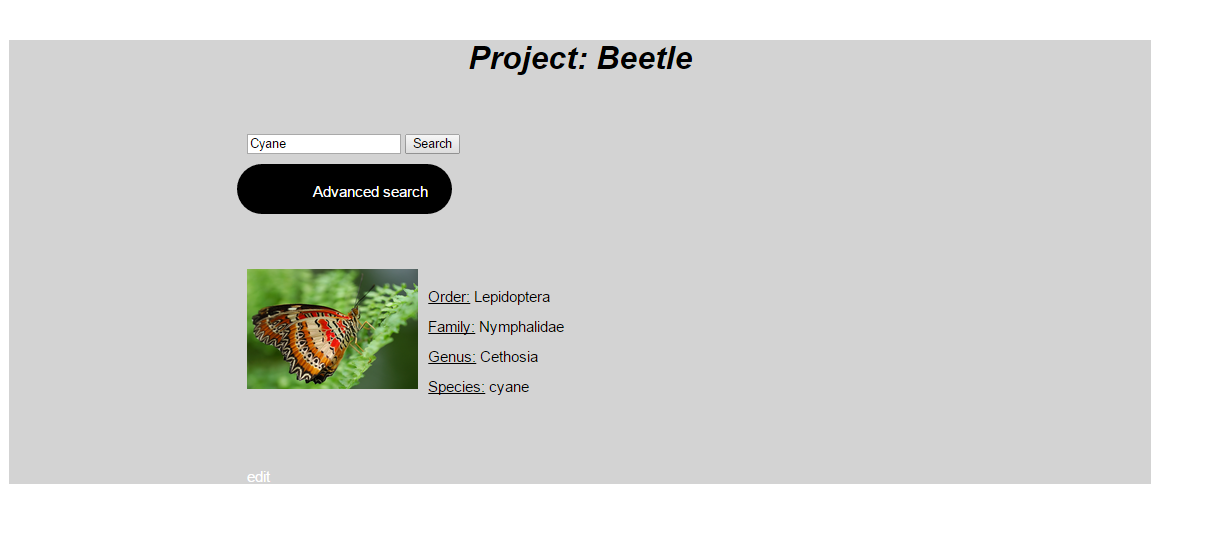
\includegraphics[height=70mm]{Prototype3.png}\\
The return of one matching entry.\\
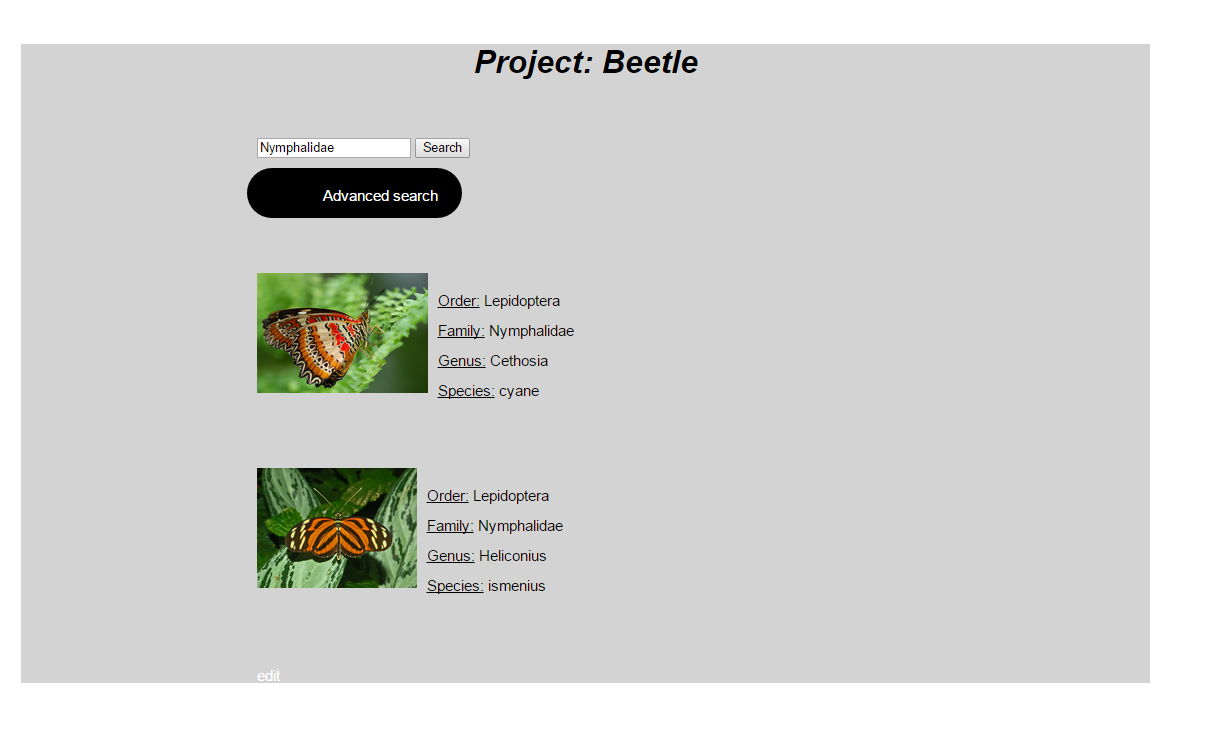
\includegraphics[height=100mm]{Prototype4.png}\\
The return of two matching entries.\\
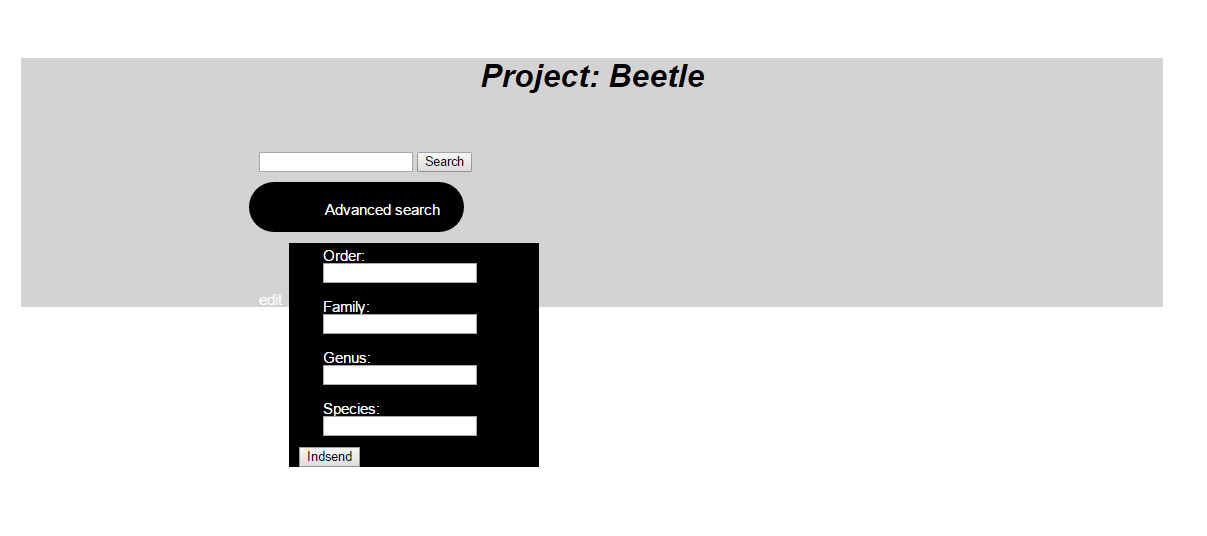
\includegraphics[height=80mm]{Prototype5.png}\\
The advanced search-engine, yet to implemented, shown by hovering your mouse over the button.\\

\newpage

\section{Internal Cooperation}
\subsection{Summary}

Come thus far, the cooperation of the University of Hamburg is satisfactory.\\
We have had a total of 3 correspondences with the client, in order to respectively request server-access, request the necessary data for establishing a correct database and to showcase the current state of our product.
All the correspondonces have been fulfilling and we will be gaining access to the server as soon as their IT-department have created a user for us.\\ Furthermore, we will be receiving the necessary data for creating the proper database the 22th of April, after which we'll have everything we need. \\
The client also expressed satisfaction regarding the current state of our product, although a desire to have it looking more akin to the current layout of their website (which is only natural given that this is a prototype).\\
Our current way of work is based on us setting up workdays and meetings depending on necessity. This means that we, rather than using a gridlocked schedule, have been deciding on days to meet when the need was expressed.\\
For organisation we have been using a group created in Skype for communication as well as a repository in Github for file-access. \\
We have been internally communicating the progress of the product along the way and have also internally decided which partials have had the most importance at a given point in time, as to ensure we are all on the same page and that deadlines will be met.\\

So far we are making great progress in the development of the product itself, and we will soon have all the available means to ensure a succesful deliverance of a working product.\\
Our effort in organising meetings and working days has been less than ideal and together with our non-gridlock scheduling style have caused us to have many subsequent days of work, causing more of a burden than what is needed.\\
In order to make our developing from here on more efficient, more emphasis will be placed on proper scheduling, in order to spread out the workload and easen the burden on the entire group. This will also allow more time for quality control.

\newpage
\section{Annexes}
\subsection{Version Control}
\subsection{Changelog}
\subsection{Timeline}



\end{document}
